% Design-of-Mach-7-nozzle-for-T4.tex
%
\documentclass[12pt,a4paper]{article}
\usepackage[body={16cm,24.5cm}]{geometry}
\usepackage{pstricks}
\usepackage{graphicx}
\usepackage{listings}
\usepackage{pdfpages}
\usepackage{subfig}
\usepackage{newapa}
\usepackage{multicol}
\lstset{basicstyle=\scriptsize,identifierstyle=,keywordstyle=}

%------------------------------------------------------------------
% a couple horizontal bars to delimit embedded code
% the width suits the page size set above and
% the mathmode eliminates spaces between the three elements
\newcommand{\topbar}{\ensuremath{
    \rule{0.1mm}{2.0mm} \rule[2.0mm]{159.5mm}{0.1mm} \rule{0.1mm}{2.0mm}
}}
\newcommand{\bottombar}{\ensuremath{
    \rule{0.1mm}{2.0mm} \rule{159.5mm}{0.1mm} \rule{0.1mm}{2.0mm}
}}
\newcommand{\topbarshort}{\ensuremath{
    \rule{0.1mm}{2.0mm} \rule[2.0mm]{149.5mm}{0.1mm} \rule{0.1mm}{2.0mm}
}}
\newcommand{\bottombarshort}{\ensuremath{
    \rule{0.1mm}{2.0mm} \rule{149.5mm}{0.1mm} \rule{0.1mm}{2.0mm}
}}
%------------------------------------------------------------------

\title{
    Flowpath design of an axisymmetric \\Mach 7.0 nozzle for T4.
}
\author{
    School of Mechanical \& Mining Engineering \\
    Research Report Number 2013/02 \\   \vspace{3mm} 
    (Also UQ HIFiRE8 Technical Report Number 2013/01) \\
    W. Y. K. Chan, M. K. Smart and P. A. Jacobs \\
    Centre for Hypersonics, The University of Queensland 
}
\date{January 2013}

\begin{document}
\maketitle

\centerline{\textbf{Abstract}}
\medskip
An axisymmetric contoured nozzle tailored for specific flight conditions
of $M\,=\,7$, $p_0\,=\,6.035$\,MPa, $T_0\,=\,2432.2$\,K has been designed 
for the T4 reflected shock tunnel facility. It has a throat diameter of 
0.021\,m and an exit diameter of 0.273166\,m, which corresponds to a 
throat-to-exit area ratio of 169.2. The nozzle has a throat-to-exit length 
of 1\,m. The nozzle produces a uniform core flow diamond with a maximum 
axial length of 1.1\,m and a maximum diameter of 0.2\,m. Cross-sectional 
flow profiles taken at the exit plane of the nozzle show that the Mach number
varies by $\pm\,0.4$\% and the flow angularity varies by $\pm\,0.13^{\circ}$.
\medskip
The initial design was based on scaling an existing nozzle that was designed
for a nearby operating condition. Starting with this scaled contour for the
supersonic part of the nozzle contour, a B\`ezier curve description of the
contour was systematically perturbed to improve the estimated test flow
conditions according to a Navier-Stokes computation that included high
temperature effects.

\newpage
\tableofcontents


%---------------------------------------------------------------------------------
\newpage
\baselineskip = 1.5pc


%---------------------------------------------------------------------------------
\section*{Nomenclature}
\label{sec:nomenclature}
\addcontentsline{toc}{section}{\numberline{}Nomenclature}

\subsection*{Roman}
\begin{multicols}{2}
 \begin{tabbing}
  XXXXXX \= \kill % This line sets the tab stop
  $a$       \> Speed of sound           \\
  $f$       \> Function                 \\
  $h$       \> Static enthalpy          \\
  $H$       \> Stagnation enthalpy      \\
  $k$       \> Turbulent kinetic energy \\
  $M$       \> Mach number              \\
  $N$       \> Number of cells          \\*[-1ex]
            \> in the core flow         \\
  $p$       \> Pressure                 \\
  $q$       \> Dynamic pressure         \\
  $r$       \> Radius                   \\
  $T$       \> Temperature              \\
  $u$       \> Axial velocity           \\
  $v$       \> Radial velocity          \\
  $x$       \> Axial distance of        \\*[-1ex]
            \> point from nozzle throat \\
  $y$, $Y$  \> Radial distance of       \\*[-1ex]
            \> point from nozzle axis   \\
 \end{tabbing}
\end{multicols}

\subsection*{Greek}
\begin{multicols}{2}
 \begin{tabbing}
  XXXXXX \= \kill % This line sets the tab stop
  $\alpha$   \> Mass fractions            \\
  $\omega$   \> Specific dissipation rate \\
  $\phi$     \> Weighting parameters      \\
  $\theta$   \> Flow angle                \\
 \end{tabbing}
\end{multicols}

\subsection*{Subscript}
\begin{multicols}{2}
 \begin{tabbing}
  XXXXXX \= \kill % This line sets the tab stop
  0          \> Total conditions         \\
  $\infty$   \> Freestream conditions    \\
  $d$        \> Design point             \\
  $s$        \> Nozzle-supply conditions \\
  $throat$   \> Throat conditions        \\
 \end{tabbing}
\end{multicols}


%---------------------------------------------------------------------------------
\newpage
\baselineskip = 1.5pc


%---------------------------------------------------------------------------------
\section{Introduction}
\label{sec:intro}
%
To facilitate the freejet testing of the HIFiRE 8 scramjet engine in the T4 shock 
tunnel facility, a new axisymmetric contoured nozzle that produces a Mach\,7 
outflow is needed. This report presents details of the design, fabrication and
testing of this new nozzle. In Section~\ref{sec:nozzle-design}, the design 
methodology that is undertaken to generate the internal flowpath of the nozzle is 
described. Section~\ref{sec:nozzle-manufacture} then summarises aspects of the 
mechanical design of the new nozzle. The technical drawings that are needed for 
the fabrication of the nozzle are included in Appendix~\ref{app:manufacturing-drawings}. 
%
%Lastly, Chapter~\ref{sec:expt-verification} 
%presents details of the experimental survey of the nozzle outflow that was 
%conducted to verify the performance of the newly-fabricated nozzle.


%---------------------------------------------------------------------------------
\section{Design methodology}
\label{sec:nozzle-design}
%
The design methodology for the new Mach\,7 nozzle follows that used by  
\shortciteB{Craddock2000} in the design of the Mach\,7.6 axisymmetric contoured 
nozzle for the T4 shock tunnel facility. This methodology involves the coupling 
of a CFD solver with an optimisation algorithm to generate a nozzle contour that
produces an outflow with the least flow angularity and the least deviations from
the desired Mach number. 

Several authors \shortcite{Korte1992,Keeling1993,Tolle1997} recommend that this 
CFD-optimiser-coupled methodology be used for the design of high Mach number 
nozzles because it generates a nozzle contour that produces a more uniform 
outflow than that designed by the conventional Method-of-Characteristics (MOC) 
methodology. In low Mach number nozzles, where boundary layers are thin, the 
location where the flow characteristics reflect is closely approximated by the 
inviscid contour as assumed by the MOC method \shortcite{Craddock2000}. However, 
for high Mach number nozzles where boundary layers are thick, the flow 
characteristics effectively reflect in the region between the wall and the 
inviscid contour, as shown in Figure~\ref{f:characteristic-lag}. This causes the 
actual reflected characteristic to lag the design reflected characteristic 
\shortcite{Candler1991}. Nozzles designed using the conventional MOC methodology 
do not account for this shift in the reflection of the flow characteristics. 
This results in the incomplete cancellation of the expansion waves in the nozzle 
which then causes the nozzle outflow to be non-uniform. On the other hand, the
CFD-optimiser-coupled methodology used in the present report incorporates a
CFD flow solver which then allows the interaction between the core flow and the 
thick boundary layer in high Mach number nozzles to be modelled correctly. 
Nozzles that are designed using this methodology are expected to produce a more 
uniform outflow.
%
\begin{figure}[htbp]
 \begin{center}
  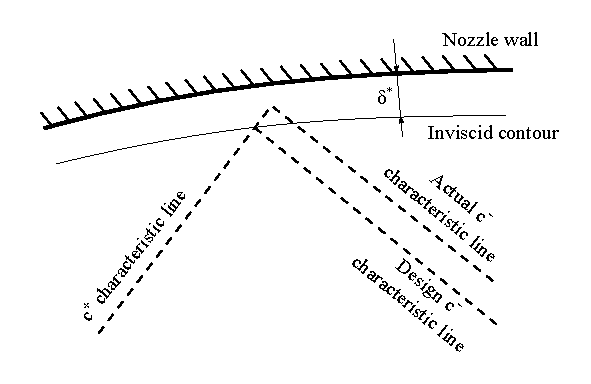
\includegraphics[width=10cm]{figs/flow-characteristic-lag.pdf}
  \caption{Lagging of the actual characteristic from the design characteristic
           due to the reflection through a thick boundary layer on the nozzle
           wall (adapted from \protect \shortciteB{Craddock2000}).}
  \label{f:characteristic-lag}
 \end{center}
\end{figure}
%

In the design of the Mach\,7.6 axisymmetric contoured nozzle for the T4 shock 
tunnel facility, \shortciteB{Craddock2000} coupled the \texttt{sm3d} CFD flow
solver with the optimisation algorithm of \shortciteB{Nelder1965}. However, 
because the \texttt{sm3d} flow solver is now obsolete, \texttt{NENZFr} is used 
instead for the design of the new Mach\,7 nozzle. \texttt{NENZFr}, which stands
for \textit{Non-Equilibrium NozZle Flow - Reloaded}, comprises of a set of 
Python scripts and template files that coordinate the running of a space-marched 
nozzle simulation using the \texttt{Eilmer3} CFD flow solver. More details on 
\texttt{NENZFr} and \texttt{Eilmer3} can be found in the reports by 
\shortciteB{Doherty2012}, \shortciteB{Jacobs2008} and \shortciteB{Jacobs2010}. 
The optimisation algorithm of Nelder \& Mead, which has already been implemented 
in the \texttt{nelmin.py} script, can be found in the \texttt{cfcfd3/lib/cfpylib/nm} 
folder in the \texttt{cfcfd3} package. Details for accessing the \texttt{cfcfd3} 
package can be found on the website \texttt{http://www.mech.uq.edu.au/cfcfd/}.


\subsection{Target nozzle-exit conditions and design constraints}
\label{sec:nozzle-design:target-conds-and-constraints}
%
The target conditions for the testing of the HIFiRE 8 engine are shown in 
Table~\ref{t:flight-test-conds}. These conditions are the target nozzle
outflow conditions for the new T4 Mach\,7 nozzle. 
%
\begin{table}[htbp]
 \begin{small}
  \begin{center}
  \caption{Target conditions for the testing of the HIFiRE 8 engine.}
  \label{t:flight-test-conds}
  \vspace{2mm}
  \begin{tabular}{@{}c@{}@{}c@{}@{}r@{}@{}l@{}|@{}c@{}@{}c@{}@{}r@{}@{}l@{}@{}c@{}}%{cccc}
  \hline\hline\noalign{\smallskip}
  \hspace{5mm} & Flow      &             &              & \hspace{5mm} & Flow      &             &             & \hspace{5mm} \\
               & parameter & \multicolumn{2}{c|}{Value} &              & parameter & \multicolumn{2}{c}{Value} &              \\
  \noalign{\smallskip}\hline\noalign{\smallskip}
  & $M_\infty$     & 7.0    &                & & $h_\infty$  & 28.56   & \,\,km  & \\
  & $q_\infty$     & 50     & \,\,kPa        & & $u_\infty$  & 2105.88 & \,\,m/s & \\
  & $H_\infty$     & 2.444  & \,\,MJ/kg\,\,  & & $a_\infty$  & 300.84  & \,\,m/s & \\
  & $p_{0,\infty}$ & 6.035  & \,\,MPa        & & $p_\infty$  & 1.4577  & \,\,kPa & \\
  & $T_{0,\infty}$ & 2432.2 & \,\,K          & & $T_\infty$  & 225.207 & \,\,K   & \\
  \noalign{\smallskip}\hline\hline
  \end{tabular}
  \end{center}
 \end{small}
\end{table}
%

In addition, there are two additional design constraints for the new Mach\,7 
nozzle. The first design constraint is that the exit diameter of the internal 
flowpath of the new nozzle has to be within +\,5\,mm of that of the existing 
Mach\,7.6 nozzle. This is to ensure that the new nozzle can utilise the same 
test-section adaptor plate as that used for the Mach\,7.6 nozzle.

The second design constraint is that of the length of the internal flowpath 
of the nozzle. The choice of the nozzle length is an important factor in the 
design of a new nozzle. For a nozzle with a fixed area ratio, a short nozzle 
means a larger expansion angle. Theoretically, the maximum divergence angle 
is given by one-half of the Prandtl-Meyer function which equates to about 
45$^{\circ}$ for a Mach\,7 flow \shortcite{Jacobs1991a}. However, large 
divergence angles will produce poor test flows because of disturbances from 
strong viscous/inviscid interactions \shortcite{Craddock1999}. Longer nozzles,
on the other hand, require longer durations to start up than short nozzles. 
This is especially disadvantageous in hypersonic impulse facilities because 
it limits the already-short test time durations. For the T4 Mach\,7.6 nozzle, 
the nozzle length of 1.11\,m was dictated by the maximum length of the 
aluminium ingot that was to be used in the manufacture of the nozzle. Since 
the chosen nozzle length for the T4 Mach\,7.6 nozzle produced a test core 
that is sufficiently large and uniform, it was decided that an initial 
estimate of the nozzle length for the new Mach\,7 nozzle can be made by 
scaling with the design Mach number. The scaled nozzle length for the new 
Mach\,7 nozzle is 1.0\,m. As shown in the numerical results in 
Section~\ref{sec:nozzle-design:optimisation-results}, the chosen nozzle length 
for the new nozzle provides a test core that is sufficiently large and uniform.


\subsection{Initial nozzle contour}
\label{sec:nozzle-design:initial-contour}
%
To start the optimisation, an initial contour for the nozzle is needed. The 
easiest way to obtain an initial contour is to scale an existing nozzle 
contour to reflect the area ratio, nozzle length and nozzle-exit diameter 
needed for the new nozzle. The other alternative is to use a MOC-generated
contour that has been corrected for the displacement thickness of the 
boundary layer that develops on the nozzle wall.

For the current study, two optimisation runs were conducted - one started with
a nozzle contour that has been geometrically scaled from the contour of the 
Mach\,7.6 nozzle\footnote{The contour of the Mach\,7.6 nozzle was scaled from
its original length of 1.11\,m to 1.0\,m. In addition, the contour was scaled
by adjusting the throat diameter (while keeping the nozzle-exit diameter constant) 
to achieve a throat-to-exit area that gave a nozzle-exit Mach number of 7.0.}, 
and the other started with a nozzle contour that has been generated by the MOC 
method and corrected for boundary layer displacement thickness. The results from 
the optimisation runs show that, by starting the optimisation from the nozzle 
contour that has been scaled from the Mach\,7.6 nozzle, the final optimised 
nozzle contour produces nozzle-exit conditions that are closer to the design 
target parameters. Only results from the optimisation run that has been started 
with the scaled nozzle contour are presented in this report.

The setup for the optimisation run for the design of the new nozzle requires 
that the initial contour be specified as design variables. This is done by 
specifying the initial contour as a B\`ezier curve with $n$ number of control 
points. The control points are obtained by fitting a B\`ezier curve to the 
initial contour using a curve-fitting code written by \shortciteB{Pastva1998}.
For the initial contour used in this study, a 7$^{th}$-degree B\`ezier curve 
was fitted to within 1$\times$10$^{-9}$\,m of the initial contour. An 
additional B\`ezier control point was also added upstream of the first control 
point to ensure that the start of the nozzle contour is parallel to the nozzle axis. 


\subsection{Determination of nozzle-throat conditions}
\label{sec:nozzle-design:nozzle-throat-conditions}
%
Another step which is required before the optimisation can be started is the 
determination of nozzle-throat conditions that would give the target conditions
at the exit of the nozzle. The nozzle-throat conditions are estimated using an
iterative process, as described.
%
\begin{enumerate}
 \item Start with an initial guess for the static pressure, static temperature 
       and flow velocity at the throat of the nozzle. These values can be 
       estimated by isentropically compressing the target nozzle-exit flow 
       given in Table~\ref{t:flight-test-conds} from Mach\,7 to Mach\,1.
 \item Use the estimated conditions as inflow conditions for a \texttt{NENZFr} 
       simulation that is set up with the parameters described in 
       Section~\ref{sec:nozzle-design:NENZFr-parameters}. 
       The nozzle contour that is used for the \texttt{NENZFr} simulation is 
       that generated in Section~\ref{sec:nozzle-design:initial-contour}.
 \item Compare the mass-flow-weighted averaged conditions in the test core at
       the nozzle-exit plane from this simulation with the target conditions 
       in Table~\ref{t:flight-test-conds}.
 \item If the values do not match, adjust the flow conditions at the throat, 
       and repeat Steps 2 and 3 until the flow conditions match. Because the
       flow encounters aerothermodynamic losses through the nozzle, the static
       pressure and static temperature at the nozzle throat has to be increased 
       (rather than decreased) for this step.
\end{enumerate}
%
The flow conditions at the throat of the nozzle that have been approximated 
using this approach are summarised in Table~\ref{t:throat-conditions}. The
flow conditions and gas composition in the nozzle-supply region, which are 
shown in Table~\ref{t:supply-conditions}, are estimated by assuming a 
hypothetical isentropic compression (occurring in thermal and chemical 
equilibrium) of the flow conditions from the nozzle throat to the 
nominally-stagnant nozzle-supply region.
%
\begin{table}[htbp]
 \begin{small}
  \begin{center}
  \caption{Estimated flow conditions at the throat of the nozzle.}
  \label{t:throat-conditions}
  \vspace{2mm}
  \begin{tabular}{@{}c@{}@{}l@{}@{}r@{}@{}l@{}@{}c@{}@{}}
  \hline\hline\noalign{\smallskip}
  \hspace{5mm}   &  Parameter \hspace{5mm}  &   \multicolumn{2}{c}{Value}  & \hspace{5mm}    \\
  \noalign{\smallskip}\hline\noalign{\smallskip}
  & $p_{throat}$    & 4.55    & \hspace{1mm} MPa   &  \\
  & $T_{throat}$    & 1861.7  & \hspace{1mm} K     &  \\
  & $u_{throat}$    & 828.8   & \hspace{1mm} m/s   &  \\
  \noalign{\smallskip}\hline\hline
  \end{tabular}
  \end{center}
 \end{small}
\end{table}
%
\begin{table}[htbp]
 \begin{small}
  \begin{center}
  \caption{Estimated flow conditions and gas compositions in the nozzle-supply region.}
  \label{t:supply-conditions}
  \vspace{2mm}
  \begin{tabular}{@{}c@{}@{}l@{}@{}r@{}@{}l@{}@{}c@{}@{}}
  \hline\hline\noalign{\smallskip}
  \hspace{5mm}   &  Parameter \hspace{5mm}  &   \multicolumn{2}{c}{Value}  & \hspace{5mm}    \\
  \noalign{\smallskip}\hline\noalign{\smallskip}
  & $p_{s}$         & 8.32    & \hspace{1mm} MPa   &  \\
  & $T_{s}$         & 2122.7  & \hspace{1mm} K     &  \\
  & $\alpha_{CO_2}$ & \multicolumn{2}{c}{0.000485}         &  \\
  & $\alpha_{NO}$   & \multicolumn{2}{c}{0.010668}         &  \\
  & $\alpha_{Ar}$   & \multicolumn{2}{c}{0.012916}         &  \\
  & $\alpha_{N_2}$  & \multicolumn{2}{c}{0.750130}         &  \\
  & $\alpha_{O_2}$  & \multicolumn{2}{c}{0.225530}         &  \\
  & $\alpha_{NO_2}$ & \multicolumn{2}{c}{0.000211}         &  \\
  \noalign{\smallskip}\hline\hline
  \end{tabular}
  \end{center}
 \end{small}
\end{table}


\subsection{Optimisation of the initial contour}
\label{sec:nozzle-design:optimisation}
%
Following \shortciteB{Craddock2000}, the optimisation problem was formulated 
using seven design variables that defined the shape of the expansion contour, 
and an objective function that defined the variation in Mach number from a 
prescribed goal and variation in flow angle across the test core at the exit 
plane of the nozzle. The radial position of the design variables were then 
optimised to minimise the objective function.

The expansion contour was described by a single continuous B\`ezier curve 
with 9 control points as shown in Figure~\ref{f:initial-contour-with-bezier-pts}.
%
\begin{figure}[htbp]
 \begin{center}
  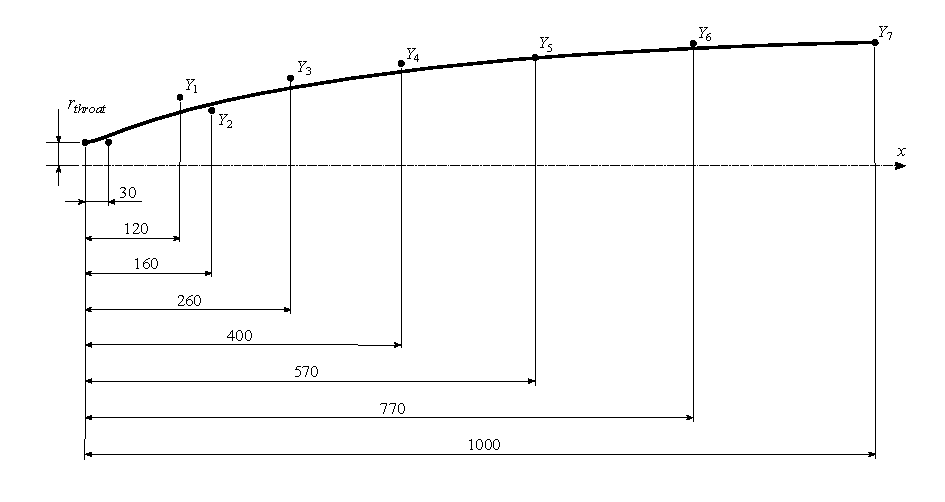
\includegraphics[width=16cm]{figs/layout-contour-bezier-pts.pdf}
  \caption{Layout of the B\`ezier control points that define the nozzle contour.}
  \label{f:initial-contour-with-bezier-pts}
 \end{center}
\end{figure}
% 
The radial positions of the first two control points were held constant at 
the nozzle throat radius and the radial positions of the remaining seven 
control points were free to move. The axial positions of all the control 
points were fixed in a distribution along the length of the nozzle that was 
slightly clustered towards the nozzle throat. The differences in radial 
distances between each pair of B\`ezier control points that were free to 
move ($Y_1 - r_{throat}$, $Y_2 - Y_1$, ....) were used as design variables. 
This approach makes the design variables resemble wall slopes and improves 
the convergence of the design procedure \shortcite{Korte1992}.

The objective function was defined so that the optimization algorithm 
would attempt to find a nozzle shape that produced a flow with a minimum 
of variation in Mach number and flow angle across the core flow at the 
nozzle-exit plane. All of the computational cells from the axis to the 
edge of the core flow\footnote{The edge of the core flow was defined as 
the radial position on the outflow plane where the gradient 
$\partial M / \partial r$  became less than $-$20.0 per metre along a radial 
line moving out from the axis (approximate edge of the boundary layer.} at the
exit plane were used to evaluate the objective function which was defined as,
%
\begin{equation}
 \label{e:objective-function}
 \mathrm{Obj} \left( dv \right) = \left( f_{\theta} + f_{M} \right)^2
\end{equation}
%

The two functions defining the variation in flow angle, $\theta$, and the 
distribution in Mach number, were
%
\begin{equation}
 \label{e:secondary-obj-function-flow-divergence}
 f_{\theta} = \frac{\phi_{\theta}^2}{N} \sum\limits_{j=1}^N \left( v_j / u_j \right)^2
\end{equation}
%
\begin{equation}
 \label{e:secondary-obj-function-Mach}
 f_{M} = \frac{\phi_{M}^2}{N} \sum\limits_{j=1}^N \left( M_{x,j} - M_{\mathrm{design}} \right)^2
 \vspace{5mm}
\end{equation}
%
where the symbol $N$ denotes the number of cells in the core flow. Two 
weighting parameters, $\phi_{\theta}$ and $\phi_M$, were used to scale the 
contributions of the flow angle variation function $f_{\theta}$ and Mach 
number variation function $f_M$. The scaling parameters were set so that both
functions would evaluate to 1 or less if all of the cells within the core flow 
have a variation in Mach number and flow angle less than a prescribed target. 
The targets were set to a variation of Mach number across the core flow at the 
exit plane of less than 0.01 and a variation of flow angularity less than 0.02$^{\circ}$,
as per those set for the design of the Mach\,7.6 nozzle by \shortciteB{Craddock2000}.
When or if the optimisation algorithm found a design solution that achieved 
these targets, the optimisation algorithm was stopped. These targets are 
``ideal'' and were set to a very high level to improve the convergence of 
the optimisation search algorithm. Note that nozzle-exit plane flow 
variations of this order can not be easily measured in pulse-flow wind 
tunnels with the current generation of flow measurement instruments.

The weighting parameters are equal to the inverse of the targets or design 
goals such that,
%
\begin{equation}
 \label{e:weighting-params-flow-divergence}
 \phi_{\theta} = \frac{1}{\mathrm{tan}\left( 0.02 \right)} = 2.86 \times 10^3
\end{equation}
%
\begin{equation}
 \label{e:weighting-params-Mach}
 \phi_{M} = \frac{1}{0.01} = 100
 \vspace{5mm}
\end{equation}
%

The initial perturbations of the design variables for the optimisation were
set to the same values as those used by \shortciteB{Craddock2000} - 3\,mm 
for the first two upstream design variables and 5\,mm for the remaining five
design variables. The parameters for the Nelder \& Mead optimiser are listed 
in Table~\ref{t:params-Nelder-Mead-opt}.
%
\begin{table}[htbp]
 \begin{small}
  \begin{center}
  \caption{Input parameters for the Nelder \& Mead optimiser.}
  \label{t:params-Nelder-Mead-opt}
  \vspace{2mm}
  \begin{tabular}{@{}c@{}@{}l@{}@{}c@{}@{}c@{}@{}c@{}@{}}
  \hline\hline\noalign{\smallskip}
  \hspace{5mm}   &  Parameter     &   \hspace{5mm} Notation \hspace{5mm}    &   Value    & \hspace{5mm}    \\
  \noalign{\smallskip}\hline\noalign{\smallskip}
  & Terminating limit for the standard                      & \texttt{tol}        &    1.0    &  \\
  & deviation of the simplex function values                &                     &           &  \\ \noalign{\smallskip}
  & Number of steps between convergence checks \hspace{5mm} & \texttt{n\_check}   &    5      &  \\ \noalign{\smallskip}
  & Maximum number of function evaluations                  & \texttt{max\_fe}    &    500    &  \\ \noalign{\smallskip}
  & Magnitude of the perturbations for                      & \texttt{delta}      &    0.001  &  \\ 
  & checking a local minimum                                &                     &           &  \\ \noalign{\smallskip}
  & Coefficient for locating new index (reflect)            & \texttt{Kreflect}   &    1.0    &  \\ \noalign{\smallskip}
  & Coefficient for locating new index (extend)             & \texttt{Kextend}    &    2.0    &  \\ \noalign{\smallskip}
  & Coefficient for locating new index (contract)           & \texttt{Kcontract}  &    0.5    &  \\
  \noalign{\smallskip}\hline\hline
  \end{tabular}
  \end{center}
 \end{small}
\end{table}
%


\subsection{NENZFr parameters}
\label{sec:nozzle-design:NENZFr-parameters}
%
The computational grid for the optimisation problem has 300 cells in the 
axial direction and 40 cells in the radial direction. As shown in 
Figure~\ref{f:NENZFr-grid}, grid clustering is employed near the throat and 
initial expansion regions to resolve the larger flow gradients expected in 
these regions. 
%
\begin{figure}[htbp]
 \begin{center}
  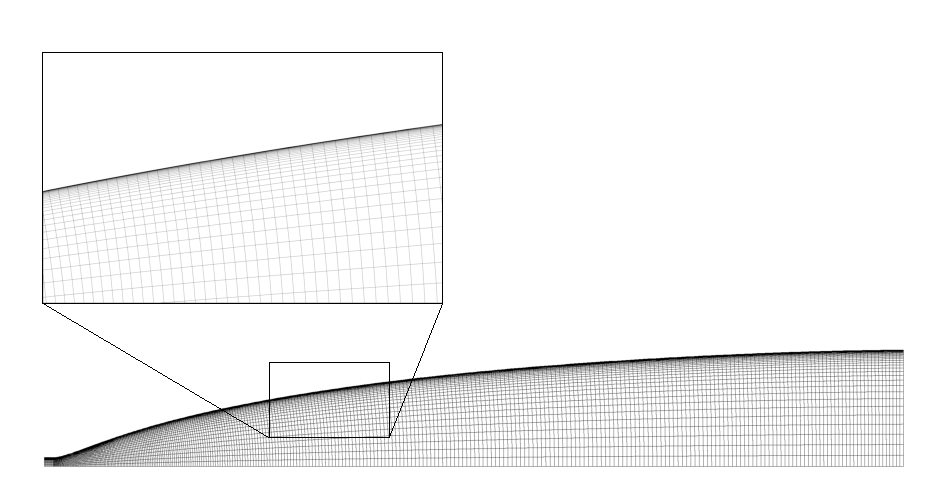
\includegraphics[width=16cm]{figs/nozzle-optimisation-grid.pdf}
  \caption{Computational grid for each \texttt{NENZFr} simulation. Close-up 
           view of the grid (displayed in the inset) shows the orthogonality 
           of the grids to the nozzle wall.}
  \label{f:NENZFr-grid}
 \end{center}
\end{figure}
%
Grid clustering is also employed near the nozzle wall to ensure sufficient 
resolution of the boundary layer. In addition, the grids near the nozzle wall 
are also configured to be orthogonal to the wall to ensure that the near-wall
flow parameters are properly approximated by flow solver. The wall of the
nozzle is assumed to be at a constant temperature of 300\,K. 

The conditions for the inflow of air through the throat of the nozzle are as 
stated in Table~\ref{t:throat-conditions}. The flow of air through the nozzle 
is assumed to be in thermal and chemical equilibrium. An additional simulation 
conducted with finite-rate chemistry showed similar results to that conducted 
with chemical equilibrium. Effects of thermal non-equilibrium flow were not 
accounted for in the simulations.

The turbulence model used in the simulations is Wilcox's 2006 $k$-$\omega$ 
turbulence model \shortcite{Wilcox2006}. The turbulence intensity of the 
inflow to the nozzle is set to 5\% and the ratio of turbulent-to-laminar 
viscosity of the inflow to the nozzle is set to 100. The resulting inflow 
turbulence kinetic energy $k$ and specific dissipation rate $\omega$ are 
derived from the turbulence intensity and the ratio of turbulent-to-laminar 
viscosity \shortcite{Chan2012a}. In addition, turbulence is assumed to start 
at the throat of the nozzle. Simulations with turbulence starting at 0\,mm, 
50\,mm, 100\,mm and 150\,mm from the throat showed that varying the transition 
location did not significantly affect the flow conditions at the exit plane of 
the nozzle (see Appendix~\ref{app:effects-BL-trans-location} for more details
on the study of the effects of varying the transition location).

To speed up the convergence of the simulations, \texttt{NENZFr} was also run 
in a multi-processor block-marching mode. More details of the block-marching 
capability is described in the report by \shortciteB{Chan2014e}.


\subsection{Optimisation results}
\label{sec:nozzle-design:optimisation-results}
%
The optimisation run converged at 115 iterations with an objective value of 
2.9. As mentioned before in Section~\ref{sec:nozzle-design:optimisation}, 
the target objective value of 1.0 was set to improve the convergence of the 
optimisation algorithm, and can only be achieved for an ideal case. It is
hence not surprising that the converged objective value for the present 
optimisation run did not reach the target objective value of 1.0. The 115 
iterations took approximately 56\,hours to complete when run parallel on 
8 Intel L5520 2.27\,GHz processors. The total number of function evaluations 
(\texttt{NENZFr} runs) was 383.

The optimised nozzle contour has a nozzle-exit diameter of 273.2\,mm. The 
maximum slope of the nozzle contour (relative to the nozzle axis) is 
20$^\circ$ and occurs approximately 42\,mm downstream of the nozzle throat.
The B\`ezier control points and physical coordinates for the optimised 
nozzle contour are shown in Table~\ref{t:Bezier-control-points} and 
Appendix~\ref{app:nozzle-coordinates} respectively. 
%
\begin{table}[htbp]
 \begin{small}
  \begin{center}
  \caption{B\`ezier control points of the optimised Mach\,7 nozzle.}
  \label{t:Bezier-control-points}
  \vspace{2mm}
  \begin{tabular}{@{}c@{}@{}c@{}@{}c@{}@{}c@{}@{}c@{}@{}}
  \hline\hline\noalign{\smallskip}
  \hspace{12mm}   &  $x$, m  &   \hspace{10mm}  & $y$, m &  \hspace{12mm} \\
  \noalign{\smallskip}\hline\noalign{\smallskip}
  & 0.000000e+00 & & 1.050000e-02 & \\
  & 3.000000e-02 & & 1.050000e-02 & \\
  & 1.200000e-01 & & 6.750100e-02 & \\
  & 1.600000e-01 & & 5.080100e-02 & \\
  & 2.600000e-01 & & 9.194200e-02 & \\
  & 4.000000e-01 & & 1.103570e-01 & \\
  & 5.700000e-01 & & 1.179570e-01 & \\
  & 7.700000e-01 & & 1.355220e-01 & \\
  & 1.000000e+00 & & 1.365830e-01 & \\
  \noalign{\smallskip}\hline\hline
  \end{tabular}
  \end{center}
 \end{small}
\end{table}
%

The radial distributions of Mach number, flow angularity, static pressure 
and Pitot pressure across the nozzle-exit plane for the optimised nozzle 
contour are shown in Figure~\ref{f:nozzle-exit-profiles}. The flow profiles
in Figure~\ref{f:nozzle-exit-profiles} are from simulations with three
grid configurations.
%
\begin{figure}[htbp]
 \begin{center}
  \subfloat[Mach number.]{
   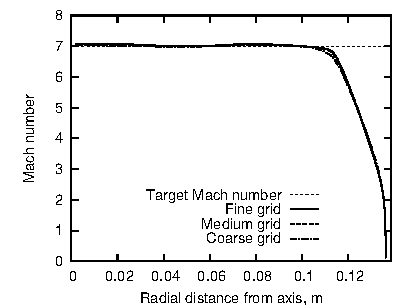
\includegraphics[width=7.9cm]{plots/profile-Mach.pdf}
   \label{f:nozzle-exit-Mach}
  }
  \subfloat[Flow angularity.]{
   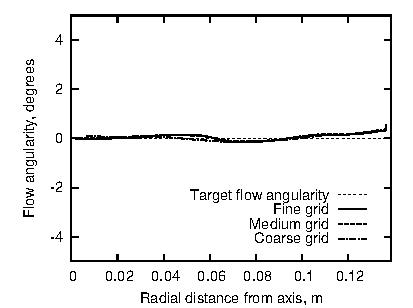
\includegraphics[width=7.9cm]{plots/profile-flow-divergence.pdf}
   \label{f:nozzle-exit-flow-angularity}
  }
  \quad
  \subfloat[Static pressure.]{
   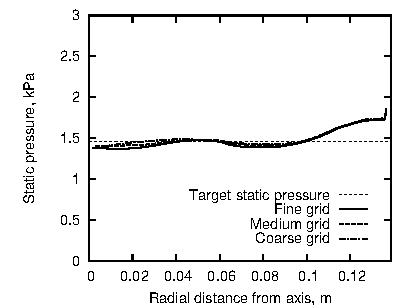
\includegraphics[width=7.9cm]{plots/profile-staticP.pdf}
   \label{f:nozzle-exit-static-pressure}
  }
  \subfloat[Pitot pressure.]{
   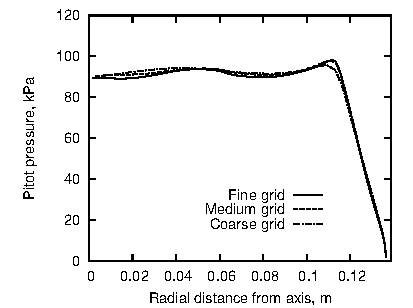
\includegraphics[width=7.9cm]{plots/profile-Pitot.pdf}
   \label{f:nozzle-exit-Pitot-pressure}
  }
  \caption{Flow profiles at the exit of the nozzle. The coarse grid, which 
           was the grid used for the optimisation run, has 40 radial cells 
           and 300 axial cells. The medium grid has 80 radial cells and 600 
           axial cells. The fine grid has 120 radial cells and 900 axial 
           cells.}
  \label{f:nozzle-exit-profiles}
 \end{center}
\end{figure}
%
These profiles show that the medium grid produces a flowfield at the 
exit of the nozzle that is sufficiently grid-converged for the analysis 
conducted in the present report (the average Mach number, flow angularity 
and Pitot pressure for the medium grid are less than 1\% different to 
those for the fine grid, while the average static pressure for the medium 
grid is 1.3\% different to that for the fine grid). As such, further 
discussions in the present report are made based on the medium grid.

The plots in Figure~\ref{f:nozzle-exit-profiles} show that, for all grid 
configurations, the maximum test core diameter at the nozzle-exit plane is 
approximately 200\,mm. Mass-flow-weighted averaged values of flow properties 
in the test core for the medium grid are summarised in 
Table~\ref{t:nozzle-exit-flow-stats}. To demonstrate the uniformity of the
nozzle-exit flow, the maximum and minimum deviations from the 
mass-flow-weighted averaged flow properties in the test core are also 
included in Table~\ref{t:nozzle-exit-flow-stats}. Other than the $\pm$\,3\%
deviation in the static pressure and the $\pm$\,2\% deviation in the Pitot
pressure, the other flow parameters have deviations of less than $\pm$\,1\%
in the test core at the nozzle-exit plane. This thus shows that flow within 
the test core is sufficiently uniform. In addition, a comparison of the
mass-flux-weighted averaged values of flow properties in the test core with
the target conditions (as shown in Table~\ref{t:flight-test-conds}) is also 
shown in Table~\ref{t:nozzle-exit-flow-stats}. The results demonstrate that 
the optimisation process produces a nozzle-exit outflow that matches to 
within 1\% of the target conditions.
%
\begin{table}[htbp]
 \begin{small}
  \begin{center}
  \caption{Mass-flow-weighted averaged values of flow properties in the 
           uniform test core. The maximum and minimum deviations from the 
           mass-flow-weighted averaged flow properties in the test core 
           are also included.}
  \label{t:nozzle-exit-flow-stats}
  \vspace{2mm}
  \begin{tabular}{@{}c@{}@{}c@{}@{}c@{}@{}c@{}@{}c@{}|@{}c@{}@{}c@{}@{}c@{}@{}c@{}@{}c@{}@{}c@{}@{}c@{}@{}c@{}@{}c@{}}
  \hline\hline\noalign{\smallskip}
  \hspace{4mm} &           &        &  Mass-flow & \hspace{3mm} & \hspace{3mm} & Max-Min    & \hspace{3mm} & Max-Min   & \hspace{4mm} &        & \hspace{4mm} & Deviation        & \hspace{4mm} \\
               & Flow      &        &  -weighted &              &              & deviation  &              & deviation &              & Target &              & from target      &              \\  
               & parameter &  Units &  value     &              &              & (absolute) &              & relative) &              & Value  &              & value (relative) &              \\
  \noalign{\smallskip}\hline\noalign{\smallskip}
               & Mach number      &    -      &  7.0215   &&& $\pm$\,0.03  &&  $\pm$\,0.4\%  &&  7.0    && +\,0.3\%          &    \\
               & Flow divergence  &  degrees  &  0.006    &&& $\pm$\,0.13  &&  -             &&  0.0    && -                 &    \\
               & Static pressure  &    kPa    &  1.4435   &&& $\pm$\,0.041 &&  $\pm$\,2.8\%  &&  1.4577 && $-$\,1.0\%        &    \\  
               & Static temperature &    K    &  223.8    &&& $\pm$\,1.9   &&  $\pm$\,0.8\%  &&  225.2  && $-$\,0.6\%        &    \\ 
               & Axial velocity   &    m/s    &  2106     &&& $\pm$\,0.9   &&  $\pm$\,0.04\% &&  2105.9 && \textless\,0.1\%  &    \\ 
               & Pitot pressure   &    kPa    &  92.324   &&& $\pm$\,1.8   &&  $\pm$\,1.9\%  &&  -      &&  -                &    \\  
  \noalign{\smallskip}\hline\hline
  \end{tabular}
  \end{center}
 \end{small}
\end{table}
%

Another parameter that is of interest is the extent of the test core that 
the optimised nozzle contour provides. Figure~\ref{f:full-simulation} shows
plots of Pitot pressure contours that are generated from simulations of the 
Mach\,7 and Mach\,7.6 nozzles and the test section of the T4 shock tunnel 
facility. Note that although this axisymmetric simulation does not model the 
true test section of the T4 shock tunnel (the actual test section has a 
square cross-section), it still does provide a reasonable estimate of the 
flowfield.
%
\begin{figure}[htbp]
 \begin{center}
  \subfloat[Mach 7 nozzle.]{
   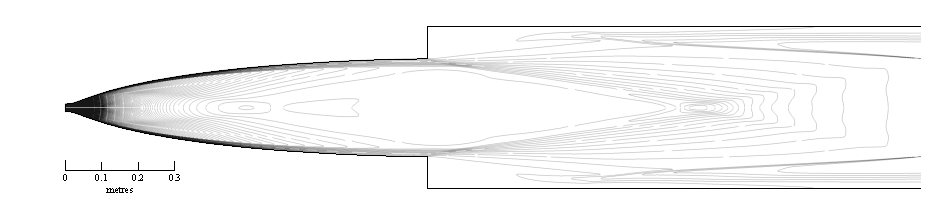
\includegraphics[width=16cm]{figs/core-flow-M7.pdf}
   \label{f:full-simulation-Mach7}
  }
  \quad
  \subfloat[Mach 7.6 nozzle.]{
   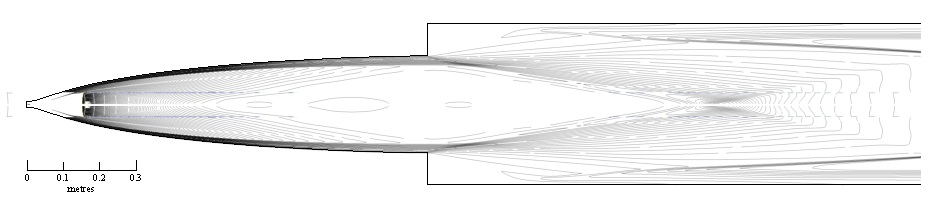
\includegraphics[width=16cm]{figs/core-flow-M8.pdf}
   \label{f:full-simulation-Mach7.6}
  }
  \caption{Contours of Pitot pressure for the Mach\,7 and the Mach\,7.6 nozzles (to scale).}
  \label{f:full-simulation}
 \end{center}
\end{figure}
%
It can be seen that the extent of core flow area is similar for both 
nozzles - the Mach\,7 nozzle produces a core flow diamond with a maximum
axial length of 1.1\,m and a maximum diameter of 0.2\,m, while the Mach\,7.6 
nozzle produces a core flow diamond with a maximum axial length of 1.2\,m and 
a maximum diameter of 0.2\,m.


%---------------------------------------------------------------------------------
\section{Manufacture}
\label{sec:nozzle-manufacture}
%
The mechanical design of the new Mach\,7 nozzle is based on that of the T4 
Mach\,7.6 nozzle. Most features of the design are kept the same, with exception to 
the following features.

\begin{itemize}
 \item The subsonic contraction and first supersonic contraction components are 
       now made from copper instead of beryllium-copper due to health and safety 
       issues related to the machining of beryllium-copper.
 \item The mechanical design and relevant o-rings for the subsonic contraction 
       and first supersonic contraction components are changed to accommodate the 
       larger throat diameter of the new Mach\,7 nozzle.
 \item The o-rings for the nozzle block, second and third supersonic expansion 
       components are changed to accommodate the different internal contour of 
       the new Mach\,7 nozzle.
\end{itemize}

This nozzle is manufactured at the UQ-EAIT workshop by Robert McGregor. The 
manufacturing drawings and details of the relevant accessories (o-rings and 
fasteners) can be found in Appendix~\ref{app:manufacturing-drawings}.


%---------------------------------------------------------------------------------
\section{Conclusion}
\label{sec:conclusion}
%
An axisymmetric contoured nozzle tailored for specific flight conditions
of $M\,=\,7$, $p_0\,=\,6.035$\,MPa, $T_0\,=\,2432.2$\,K has been designed 
for the T4 reflected shock tunnel facility. It has a throat diameter of 
0.021\,m and an exit diameter of 0.273166\,m, which corresponds to a 
throat-to-exit area ratio of 169.2. The nozzle has a throat-to-exit length 
of 1\,m. The nozzle produces a uniform core flow diamond with a maximum 
axial length of 1.1\,m and a maximum diameter of 0.2\,m. Cross-sectional 
flow profiles taken at the exit plane of the nozzle show that the Mach number
varies by $\pm\,0.4$\% and the flow angularity varies by $\pm\,0.13^{\circ}$.


\newpage
\bibliography{../phd_bibliography}
\bibliographystyle{newapa}  % When using newapa bib style, remember to include
                            % \usepackage{newapa} in the preamble.

\newpage


%---------------------------------------------------------------------------------
\appendix

%---------------------------------------------------------------------------------
\newpage
\section{Optimisation script (.py)}
\label{app:optimisation-script}
\topbar
\lstinputlisting[language={}]{scripts/optimise_nozzle.py}
\bottombar

%---------------------------------------------------------------------------------
\newpage
\section{Effects of varying boundary layer transitioning location}
\label{app:effects-BL-trans-location}
%
This appendix presents an investigation into how differences in the location where 
boundary layer transitions in the Mach\,7 nozzle can affect the flow quality at 
the exit of the nozzle. \texttt{NENZFr} simulations of the optimised Mach\,7 nozzle 
with boundary layer transitioning locations at 0\,mm, 50\,mm, 100\,mm and 150\,mm 
from the throat are performed. Figure~\ref{f:nozzle-exit-profiles-effects-BL-trans}
%
\begin{figure}[htbp]
 \begin{center}
  \subfloat[Mach number.]{
   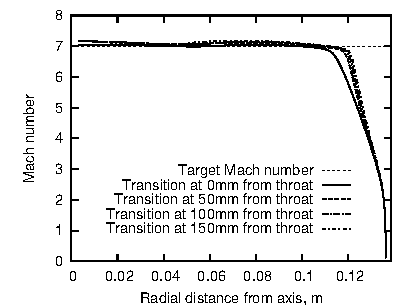
\includegraphics[width=7.9cm]{plots/effects-BL-trans-Mach.pdf}
   \label{f:nozzle-exit-Mach-effects-BL-trans}
  }
  \subfloat[Flow angularity.]{
   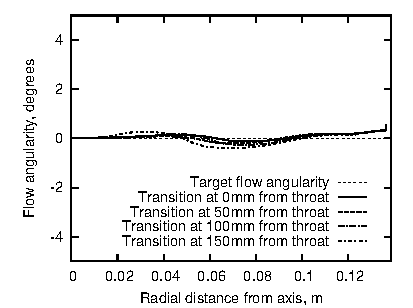
\includegraphics[width=7.9cm]{plots/effects-BL-trans-flow-divergence.pdf}
   \label{f:nozzle-exit-flow-angularity-effects-BL-trans}
  }
  \quad
  \subfloat[Static pressure.]{
   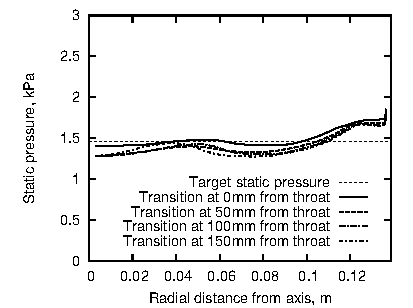
\includegraphics[width=7.9cm]{plots/effects-BL-trans-staticP.pdf}
   \label{f:nozzle-exit-static-pressure-effects-BL-trans}
  }
  \subfloat[Pitot pressure.]{
   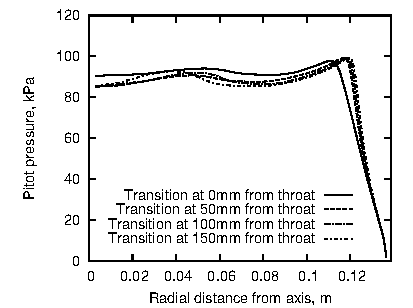
\includegraphics[width=7.9cm]{plots/effects-BL-trans-Pitot.pdf}
   \label{f:nozzle-exit-Pitot-pressure-effects-BL-trans}
  }
  \caption{Flow profiles at the exit of the nozzle for simulations with
           boundary layer transitioning locations at 0\,mm, 50\,mm, 
           100\,mm and 150\,mm from the throat.}
  \label{f:nozzle-exit-profiles-effects-BL-trans}
 \end{center}
\end{figure}
% 
shows the flow profiles that have been extracted from these simulations at the exit 
plane of the nozzle. These profiles show that the more downstream the boundary layer 
transitions to turbulence, the thinner the boundary layer will be, which then 
results in a higher nozzle-exit Mach number, a lower nozzle-exit static pressure and 
a lower nozzle-exit Pitot pressure. In addition, the flow angularity also becomes 
higher when the boundary layer transitioning location is shifted downstream of the 
throat.

Figure~\ref{f:nozzle-exit-profiles-quantify-effects-BL-trans} shows the percentage 
deviation of nozzle-exit flow properties (for simulations with the boundary layer  
%
\begin{figure}[htbp]
 \begin{center}
  \subfloat[Mach number.]{
   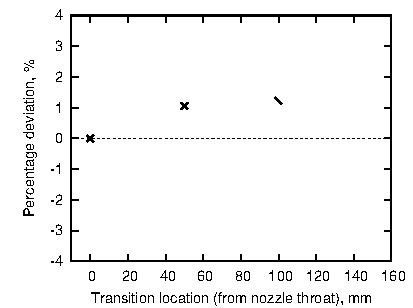
\includegraphics[width=7.9cm]{plots/quantify-effects-BL-trans-Mach.pdf}
   \label{f:nozzle-exit-Mach-quantify-effects-BL-trans}
  }
  \subfloat[Static temperature.]{
   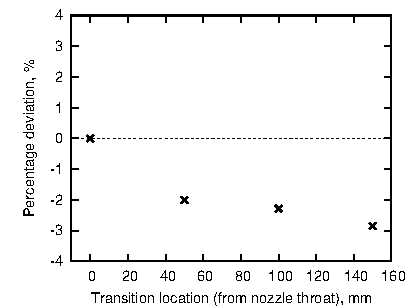
\includegraphics[width=7.9cm]{plots/quantify-effects-BL-trans-temperature.pdf}
   \label{f:nozzle-exit-temperature-quantify-effects-BL-trans}
  }
  \quad
  \subfloat[Static density.]{
   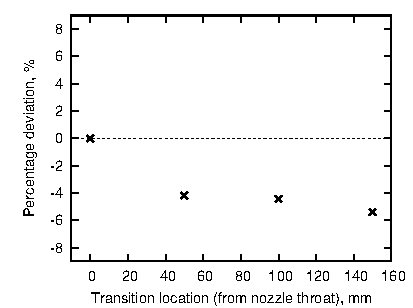
\includegraphics[width=7.9cm]{plots/quantify-effects-BL-trans-density.pdf}
   \label{f:nozzle-exit-density-quantify-effects-BL-trans}
  }
  \subfloat[Axial velocity.]{
   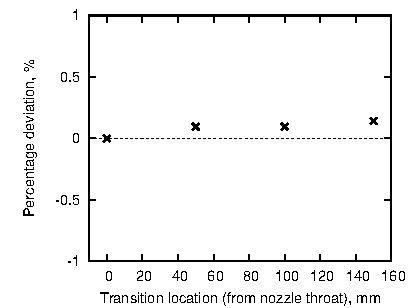
\includegraphics[width=7.9cm]{plots/quantify-effects-BL-trans-x-vel.pdf}
   \label{f:nozzle-exit-x-vel-quantify-effects-BL-trans}
  }
  \quad
  \subfloat[Static pressure.]{
   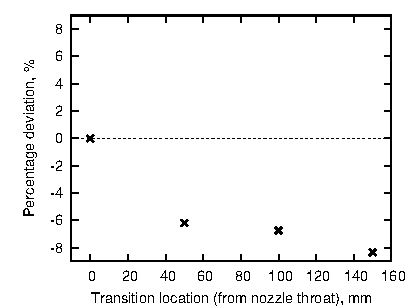
\includegraphics[width=7.9cm]{plots/quantify-effects-BL-trans-pressure.pdf}
   \label{f:nozzle-exit-static-pressure-quantify-effects-BL-trans}
  }
  \subfloat[Pitot pressure.]{
   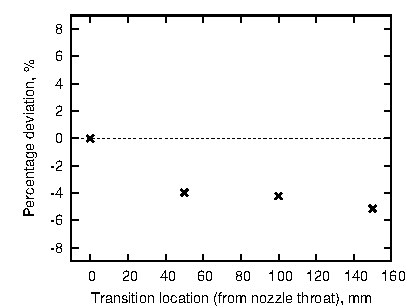
\includegraphics[width=7.9cm]{plots/quantify-effects-BL-trans-Pitot.pdf}
   \label{f:nozzle-exit-Pitot-pressure-quantify-effects-BL-trans}
  }
  \caption{Percentage deviation of nozzle-exit flow properties for simulations 
           with the boundary layer transitioning location set at 50\,mm, 100\,mm 
           and 150\,mm from those for simulations with the boundary layer 
           transitioning at the throat. The percentage deviation is computed using
           Equation~\ref{e:percent-deviation}. Note that the flow properties are 
           mass-flow-weighted averaged values of properties at the exit of the nozzle.}
  \label{f:nozzle-exit-profiles-quantify-effects-BL-trans}
 \end{center}
\end{figure}
%
transitioning location set at 50\,mm, 100\,mm and 150\,mm) from those for simulations 
with the boundary layer transitioning at the throat. The percentage deviation is 
computed by 
%
\begin{equation}
 \% \, \mathrm{deviation} \, = \, \frac{|X - X_{throat}|}{X_{throat}} \, \times \, 100\%
 \label{e:percent-deviation}
\end{equation}
%
where $X$ is the nozzle-exit flow property. These results show that for transitioning
locations up to 150\,mm from the throat, the maximum deviation from that when 
boundary layer transitioning occurs at the throat is $+0.2$\% for nozzle-exit 
velocity, $+1.5$\% for nozzle-exit Mach number, $-3$\% for nozzle-exit static 
temperature, $-5$\% for nozzle-exit Pitot pressure and nozzle-exit static density, 
and $-8$\% for nozzle-exit static pressure. For transitioning locations up to 150\,mm 
from the throat, most flow variables at the exit of the nozzle (other than the static 
pressure) are not significantly affected by differences in the location where the 
boundary layer transitions to turbulence.

%---------------------------------------------------------------------------------
\newpage
\section{Coordinates for the nozzle contour}
\label{app:nozzle-coordinates}
%
The coordinates for the Mach\,7 nozzle contour are listed here. For users
who would like to use these coordinates for either their CFD simulations or for
manufacturing purposes, the authors highly recommend that the coordinates be 
taken from the master copy \texttt{contour-t4-m7.data} which can be located in the 
\texttt{cfcfd3/app/nenzfr/nenzfr\_data\_files/} folder in the cfcfd3 package. Details
for accessing the \texttt{cfcfd3} package can be found on 
\texttt{http://www.mech.uq.edu.au/cfcfd/index.html}. This is to avoid having
multiple master copies of the coordinates data.
%
\vspace{5mm}
\lstinputlisting[language={}]{nozzle-contour-data/contour-t4-m7.data}

%---------------------------------------------------------------------------------
\newpage
\section{Manufacturing drawings}
\label{app:manufacturing-drawings}

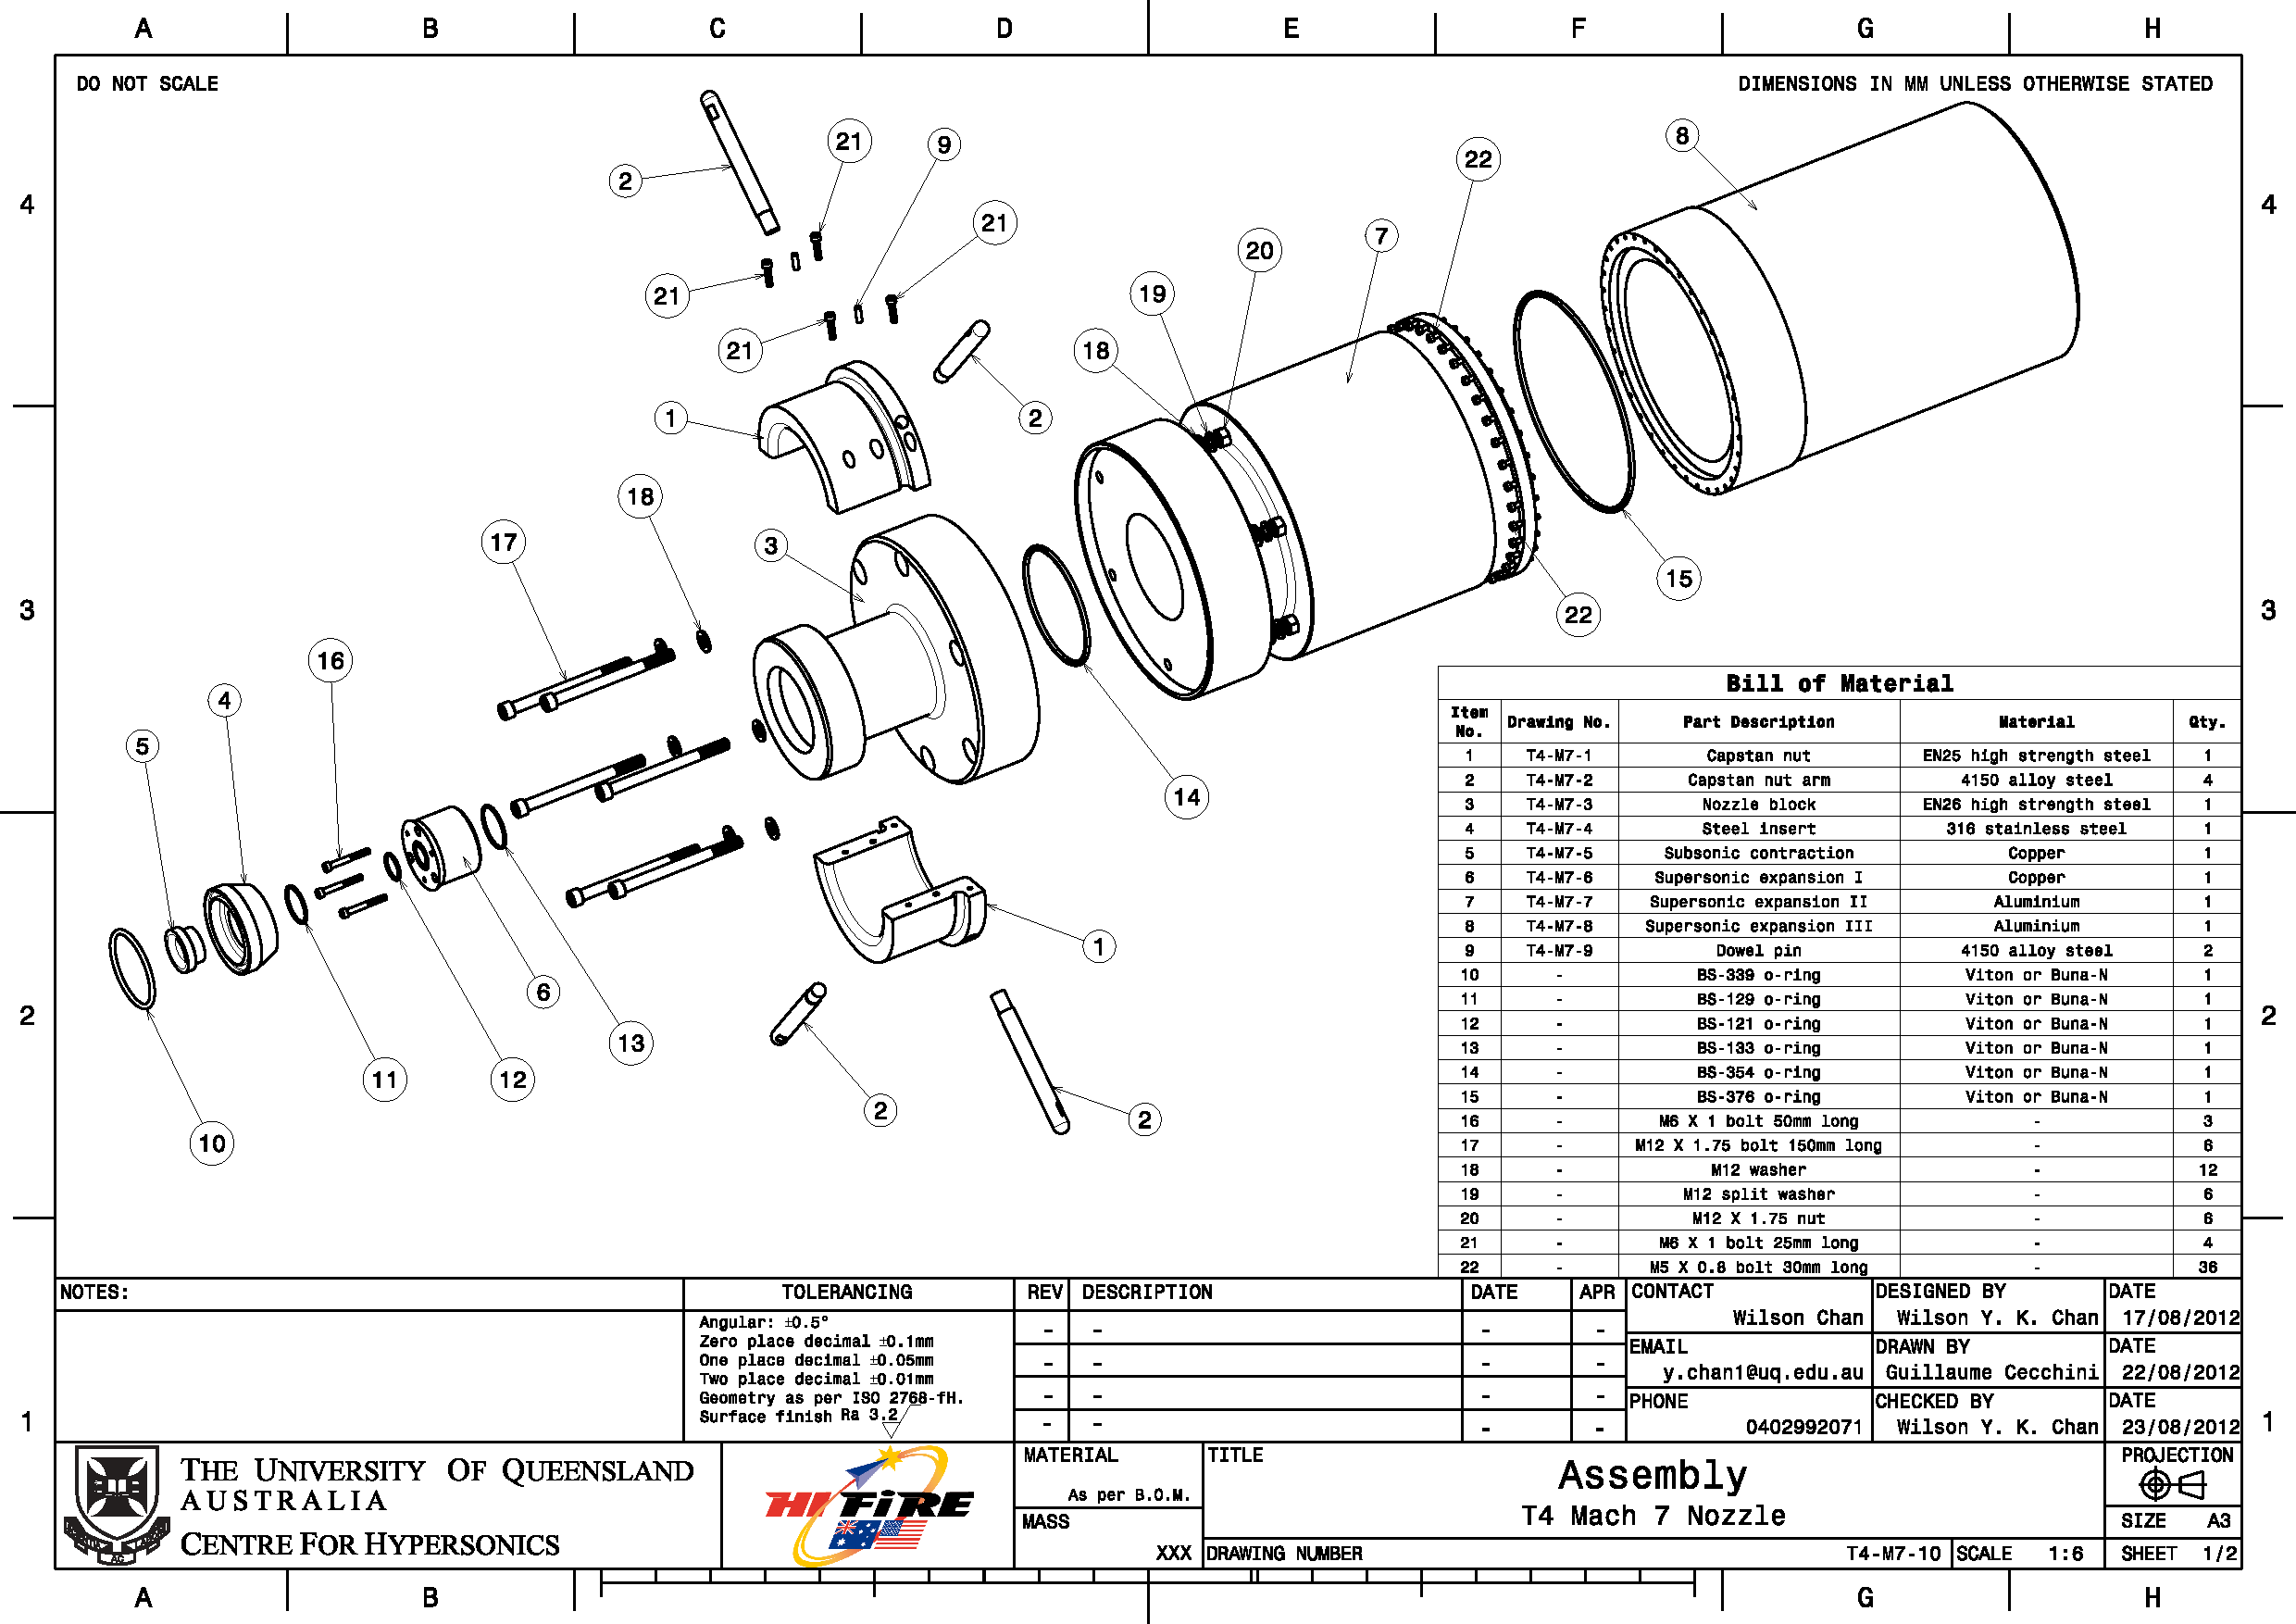
\includepdf[landscape]{../../project-Mach-7-nozzle/CAD-M7-nozzle/T4-M7-Nozzle-Drawings/T4-M7-10_Sheet_1.pdf}

\includepdf[landscape]{../../project-Mach-7-nozzle/CAD-M7-nozzle/T4-M7-Nozzle-Drawings/T4-M7-10_Sheet_2.pdf}

\includepdf[landscape]{../../project-Mach-7-nozzle/CAD-M7-nozzle/T4-M7-Nozzle-Drawings/T4-M7-1_Sheet_1.pdf}

\includepdf[landscape]{../../project-Mach-7-nozzle/CAD-M7-nozzle/T4-M7-Nozzle-Drawings/T4-M7-1_Sheet_2.pdf}

\includepdf[landscape]{../../project-Mach-7-nozzle/CAD-M7-nozzle/T4-M7-Nozzle-Drawings/T4-M7-2.pdf}

\includepdf[landscape]{../../project-Mach-7-nozzle/CAD-M7-nozzle/T4-M7-Nozzle-Drawings/T4-M7-3_Sheet_1.pdf}

\includepdf[landscape]{../../project-Mach-7-nozzle/CAD-M7-nozzle/T4-M7-Nozzle-Drawings/T4-M7-3_Sheet_2.pdf}

\includepdf[landscape]{../../project-Mach-7-nozzle/CAD-M7-nozzle/T4-M7-Nozzle-Drawings/T4-M7-4.pdf}

\includepdf[landscape]{../../project-Mach-7-nozzle/CAD-M7-nozzle/T4-M7-Nozzle-Drawings/T4-M7-5.pdf}

\includepdf[landscape]{../../project-Mach-7-nozzle/CAD-M7-nozzle/T4-M7-Nozzle-Drawings/T4-M7-6.pdf}
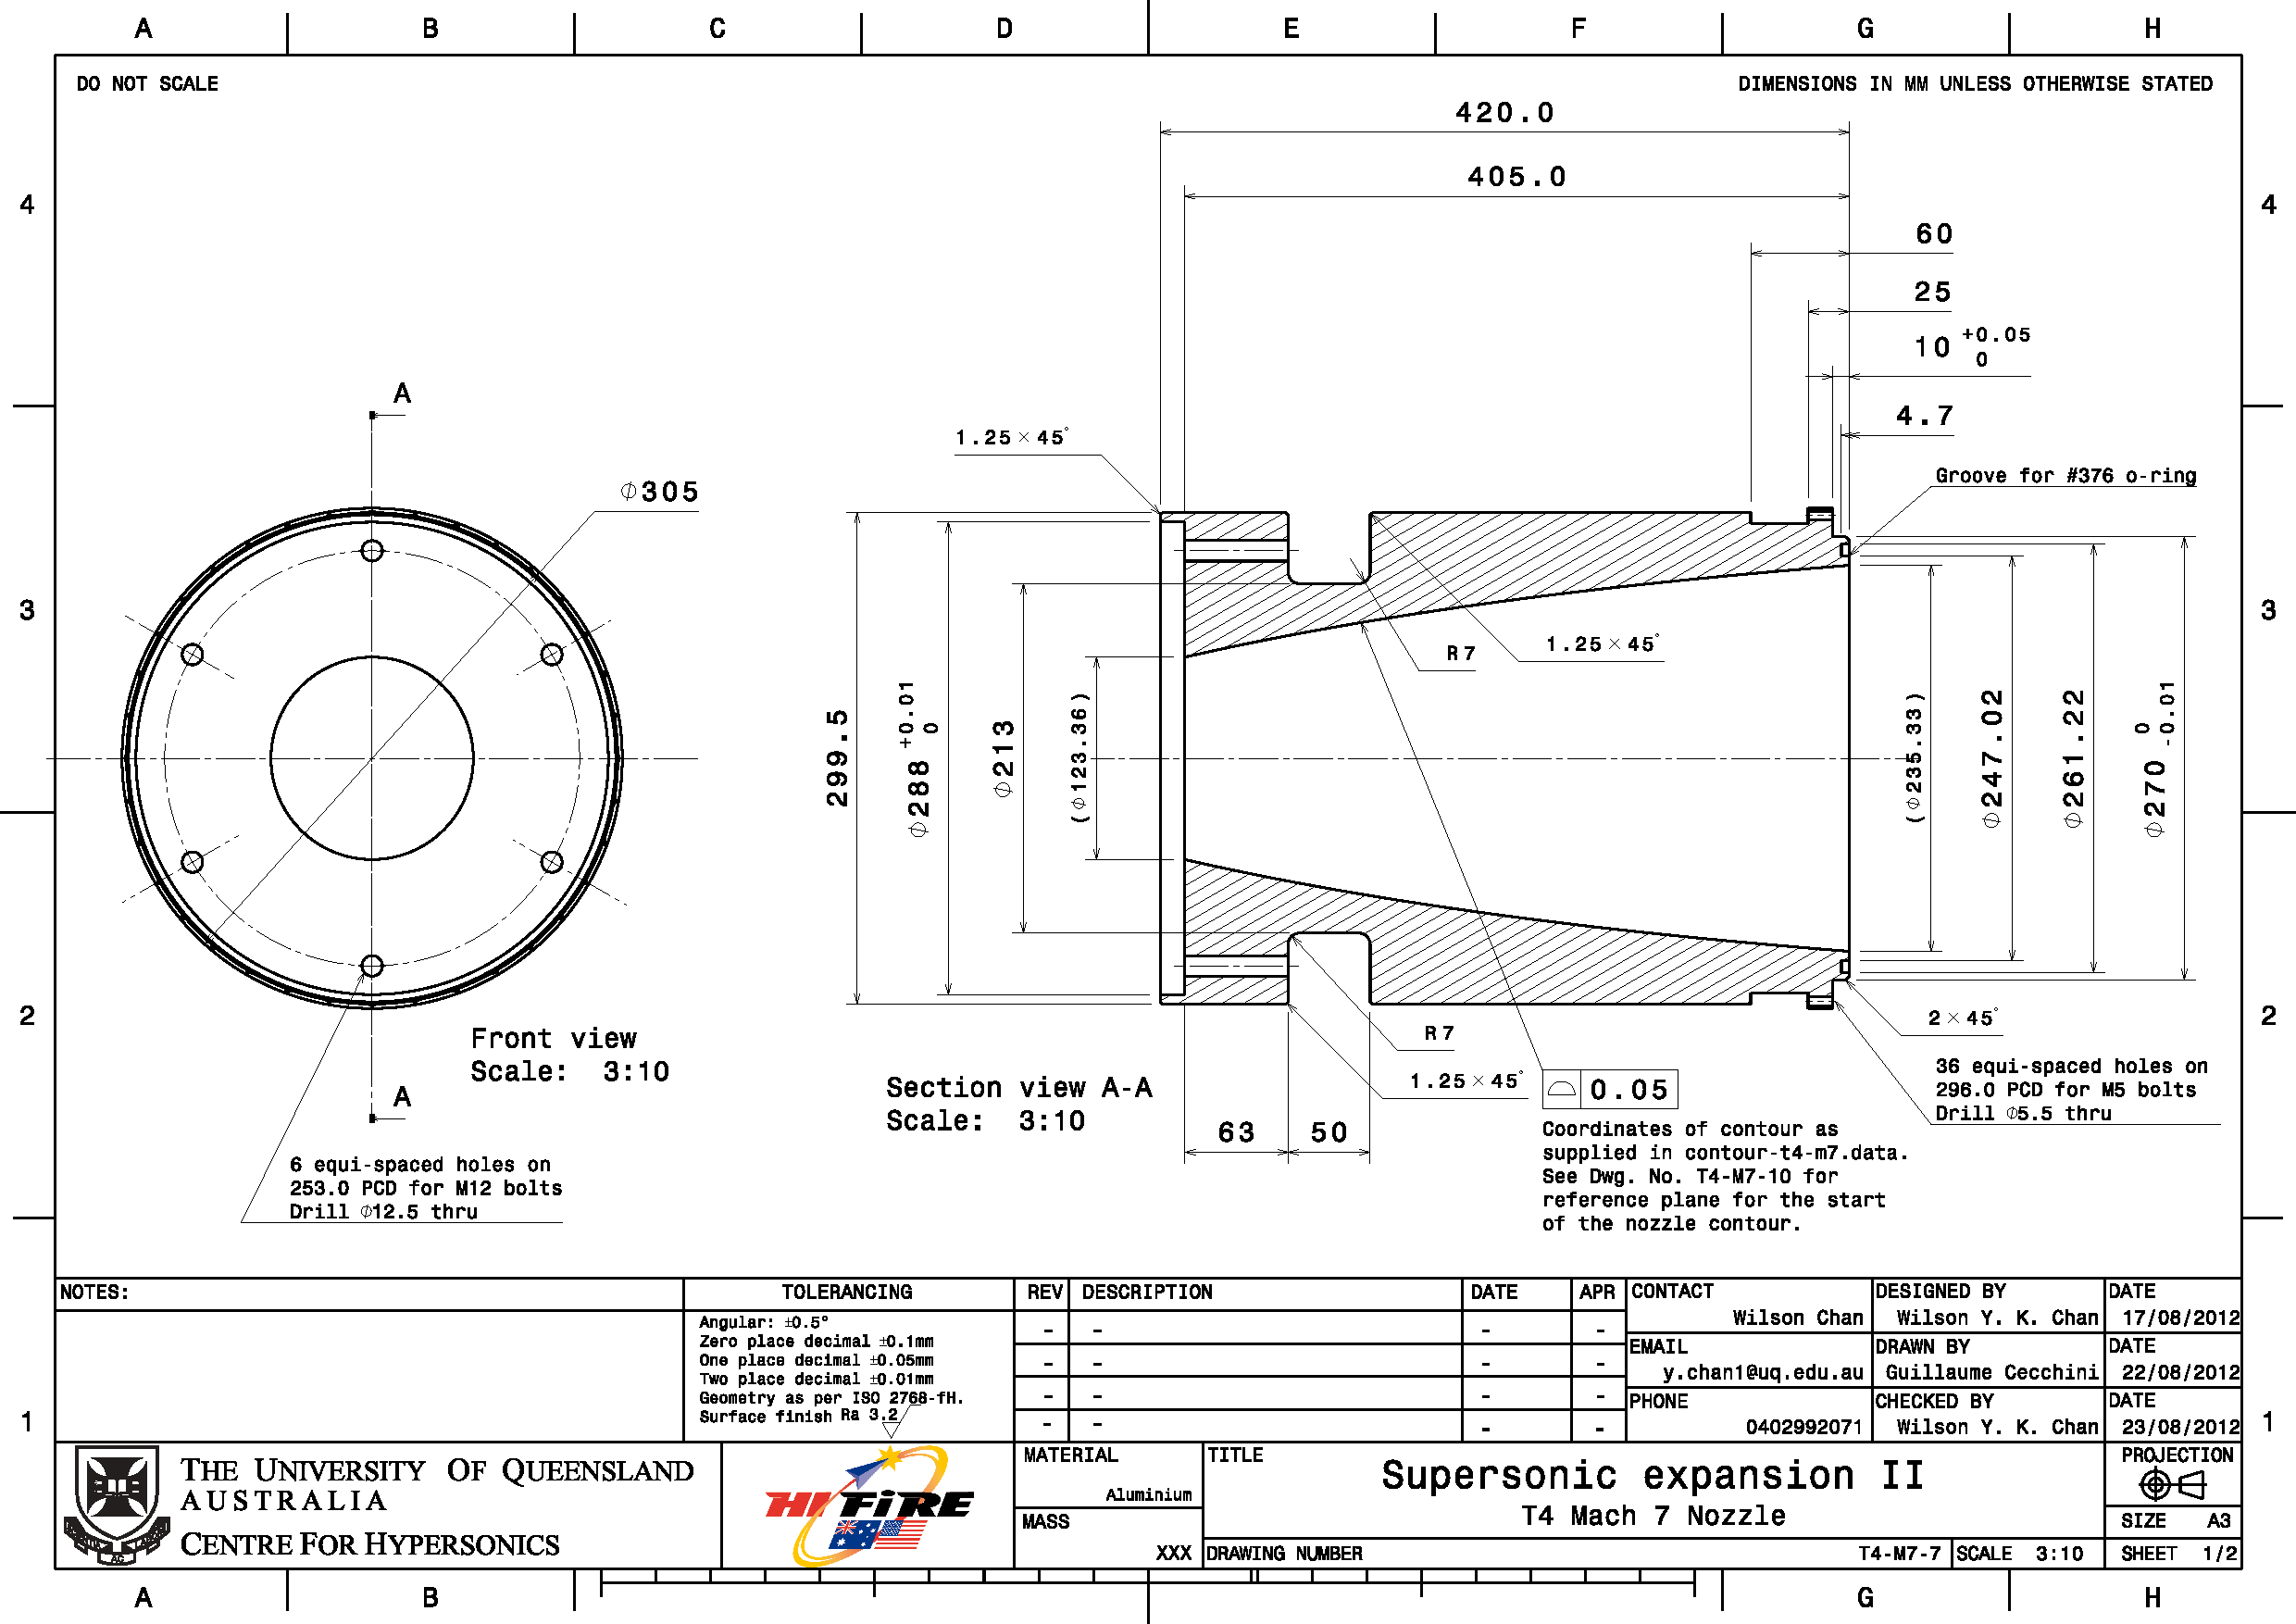
\includepdf[landscape]{../../project-Mach-7-nozzle/CAD-M7-nozzle/T4-M7-Nozzle-Drawings/T4-M7-7_Sheet_1.pdf}

\includepdf[landscape]{../../project-Mach-7-nozzle/CAD-M7-nozzle/T4-M7-Nozzle-Drawings/T4-M7-7_Sheet_2.pdf}
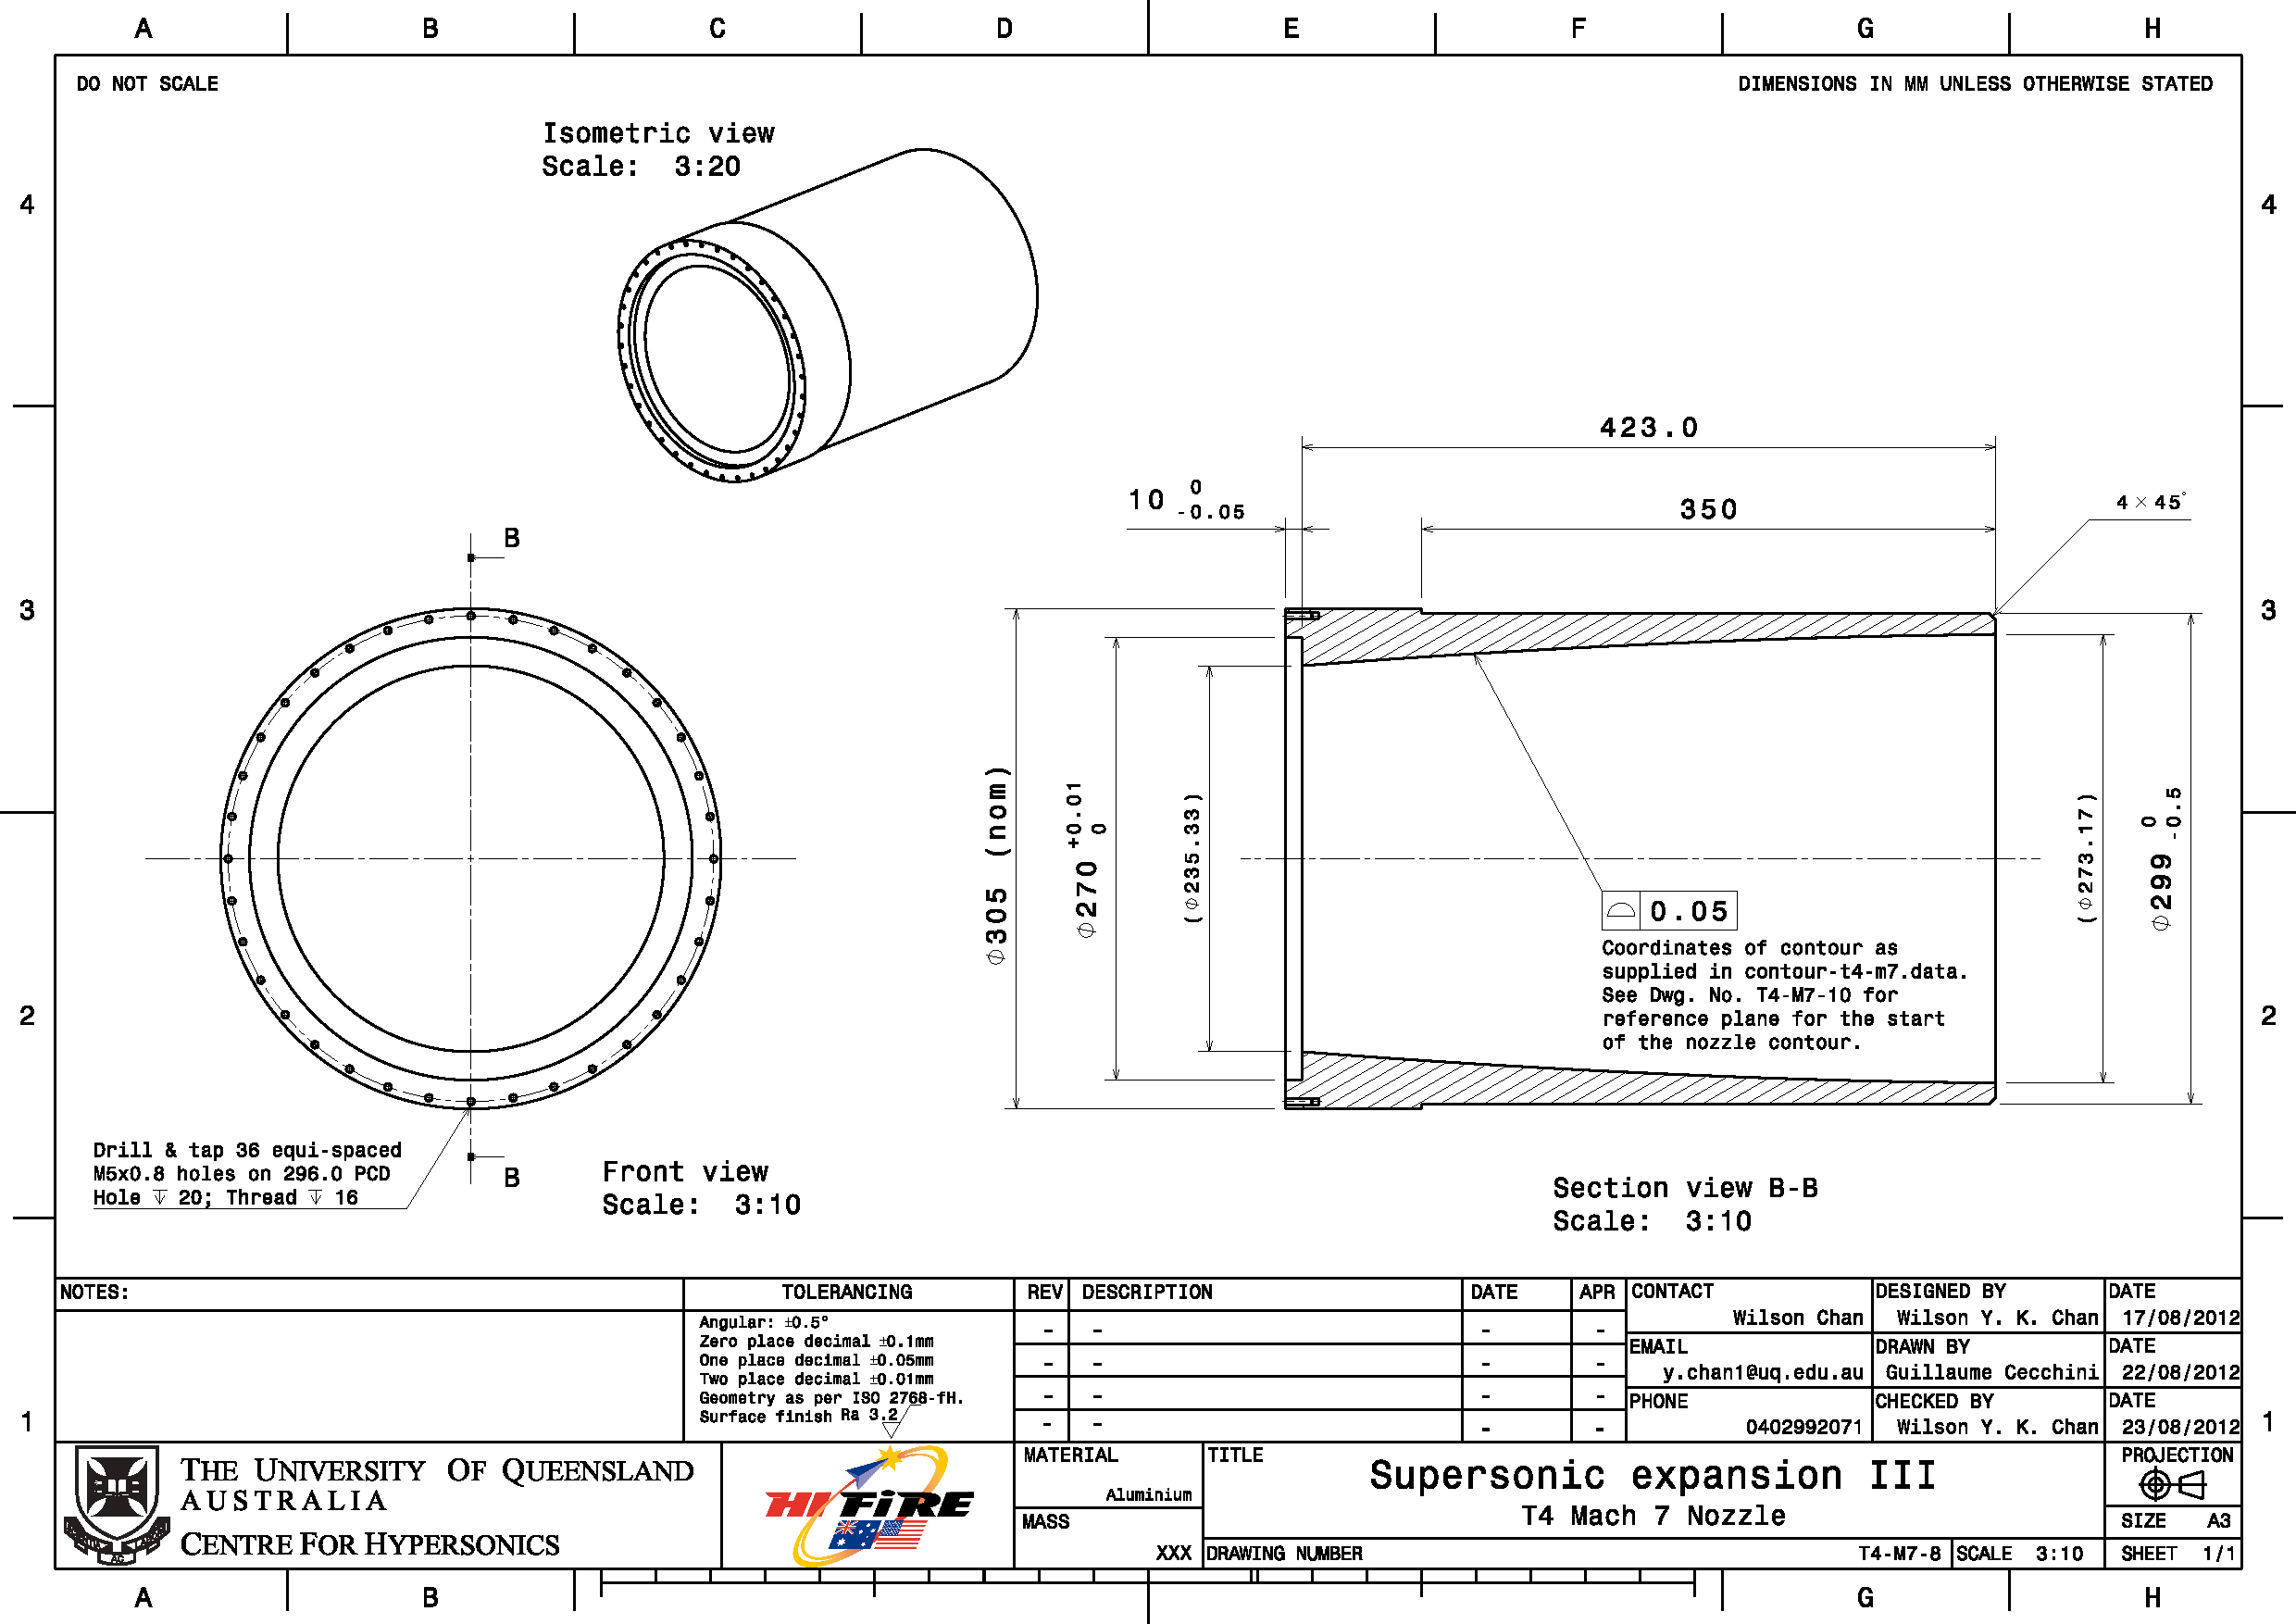
\includepdf[landscape]{../../project-Mach-7-nozzle/CAD-M7-nozzle/T4-M7-Nozzle-Drawings/T4-M7-8.pdf}

\includepdf[landscape]{../../project-Mach-7-nozzle/CAD-M7-nozzle/T4-M7-Nozzle-Drawings/T4-M7-9.pdf}

%---------------------------------------------------------------------------------


\end{document}
